\documentclass{article}
\usepackage{graphicx}
\usepackage[margin=1.5cm]{geometry}
\usepackage{amsmath}

\begin{document}

\title{Wednesday Reading Assessment: Unit 2}
\author{Prof. Jordan C. Hanson}

\maketitle

\section{Chapter 4 - Kinematics in Two and Three Dimensions}

\begin{figure}[ht]
\centering
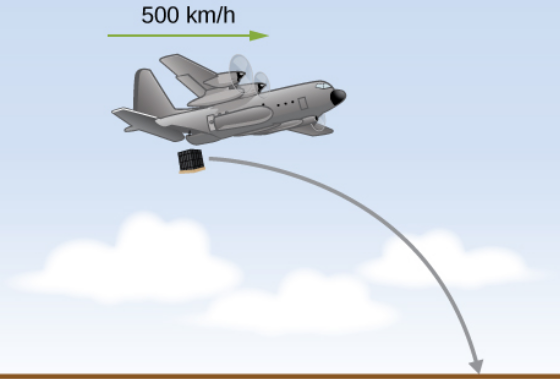
\includegraphics[width=0.3\textwidth]{plane.png}
\end{figure}

\begin{enumerate}
\item An airplane flying horizontally with a speed of 140 m/s at a height of 800 m drops a crate of supplies.  If the parachute fails to open, how far in front of the release point does the crate hit the ground? \\ \vspace{5cm}
\item Suppose the airplane in the preceding problem instead launches the crate horizontally in its direction of motion at a speed of 100 m/s in addition to the speed of the plane.  Where will the create land?
\end{enumerate}

\end{document}
